%% History:
% Pavel Tvrdik (26.12.2004)
%  + initial version for PhD Report
%
% Daniel Sykora (27.01.2005)
%
% Michal Valenta (3.12.2008)
% rada zmen ve formatovani (diky M. Duškovi, J. Holubovi a J. Žďárkovi)
% sjednoceni zdrojoveho kodu pro anglickou, ceskou, bakalarskou a diplomovou praci

% One-page layout: (proof-)reading on display
%%%% \documentclass[11pt,oneside,a4paper]{book}
% Two-page layout: final printing
\documentclass[11pt,twoside,a4paper]{book}   
%=-=-=-=-=-=-=-=-=-=-=-=--=%
% The user of this template may find useful to have an alternative to these 
% officially suggested packages:
\usepackage[czech, english]{babel}
%\usepackage[T1]{fontenc} % pouzije EC fonty 
% pripadne pisete-li cesky, pak lze zkusit take:
\usepackage[OT1]{fontenc} 
\usepackage[utf8]{inputenc}
%=-=-=-=-=-=-=-=-=-=-=-=--=%
% In case of problems with PDF fonts, one may try to uncomment this line:
%\usepackage{lmodern}
%=-=-=-=-=-=-=-=-=-=-=-=--=%
%=-=-=-=-=-=-=-=-=-=-=-=--=%
% Depending on your particular TeX distribution and version of conversion tools 
% (dvips/dvipdf/ps2pdf), some (advanced | desperate) users may prefer to use 
% different settings.
% Please uncomment the following style and use your CSLaTeX (cslatex/pdfcslatex) 
% to process your work. Note however, this file is in UTF-8 and a conversion to 
% your native encoding may be required. Some settings below depend on babel 
% macros and should also be modified. See \selectlanguage \iflanguage.
%\usepackage{czech}  %%%%%\usepackage[T1]{czech} %%%%[IL2] [T1] [OT1]
%=-=-=-=-=-=-=-=-=-=-=-=--=%

%%%%%%%%%%%%%%%%%%%%%%%%%%%%%%%%%%%%%%%
% Styles required in your work follow %
%%%%%%%%%%%%%%%%%%%%%%%%%%%%%%%%%%%%%%%
\usepackage{graphicx}
%\usepackage{indentfirst} %1. odstavec jako v cestine.

\usepackage{k336_thesis_macros} % specialni makra pro formatovani DP a BP
 % muzete si vytvorit i sva vlastni v souboru k336_thesis_macros.sty
 % najdete  radu jednoduchych definic, ktere zde ani nejsou pouzity
 % napriklad: 
 % \newcommand{\bfig}{\begin{figure}\begin{center}}
 % \newcommand{\efig}{\end{center}\end{figure}}
 % umoznuje pouzit prikaz \bfig namisto \begin{figure}\begin{center} atd.


%%%%%%%%%%%%%%%%%%%%%%%%%%%%%%%%%%%%%
% Zvolte jednu z moznosti 
% Choose one of the following options
%%%%%%%%%%%%%%%%%%%%%%%%%%%%%%%%%%%%%
% \newcommand\TypeOfWork{Diplomová práce} \typeout{Diplomova prace}
% \newcommand\TypeOfWork{Master's Thesis}   \typeout{Master's Thesis} 
\newcommand\TypeOfWork{Bakalářská práce}  \typeout{Bakalarska prace}
% \newcommand\TypeOfWork{Bachelor's Project}  \typeout{Bachelor's Project}


%%%%%%%%%%%%%%%%%%%%%%%%%%%%%%%%%%%%%
% Zvolte jednu z moznosti 
% Choose one of the following options
%%%%%%%%%%%%%%%%%%%%%%%%%%%%%%%%%%%%%
% nabidky jsou z: http://www.fel.cvut.cz/cz/education/bk/prehled.html

%\newcommand\StudProgram{Elektrotechnika a informatika, dobíhající, Bakalářský}
%\newcommand\StudProgram{Elektrotechnika a informatika, dobíhající, Magisterský}
% \newcommand\StudProgram{Elektrotechnika a informatika, strukturovaný, Bakalářský}
% \newcommand\StudProgram{Elektrotechnika a informatika, strukturovaný, Navazující magisterský}
\newcommand\StudProgram{Softwarové technologie a management}
% English study:
% \newcommand\StudProgram{Electrical Engineering and Information Technology}  % bachelor programe
% \newcommand\StudProgram{Electrical Engineering and Information Technology}  %master program


%%%%%%%%%%%%%%%%%%%%%%%%%%%%%%%%%%%%%
% Zvolte jednu z moznosti 
% Choose one of the following options
%%%%%%%%%%%%%%%%%%%%%%%%%%%%%%%%%%%%%
% nabidky jsou z: http://www.fel.cvut.cz/cz/education/bk/prehled.html

%\newcommand\StudBranch{Výpočetní technika}   % pro program EaI bak. (dobihajici i strukt.)
%\newcommand\StudBranch{Výpočetní technika}   % pro prgoram EaI mag. (dobihajici i strukt.)
%\newcommand\StudBranch{Softwarové inženýrství}            %pro STM
\newcommand\StudBranch{Web a multimedia}                  % pro STM
%\newcommand\StudBranch{Computer Engineering}              % bachelor programe
%\newcommand\StudBranch{Computer Science and Engineering}  % master programe


%%%%%%%%%%%%%%%%%%%%%%%%%%%%%%%%%%%%%%%%%%%%
% Vyplnte nazev prace, autora a vedouciho
% Set up Work Title, Author and Supervisor
%%%%%%%%%%%%%%%%%%%%%%%%%%%%%%%%%%%%%%%%%%%%

\newcommand\WorkTitle{Návrh ontologie pro přehrávač hudby}
\newcommand\FirstandFamilyName{Martin Doubravský}
\newcommand\Supervisor{Ing. Ladislav Kunc}


% Pouzijete-li pdflatex, tak je prijemne, kdyz bude mit vase prace
% funkcni odkazy i v pdf formatu
\usepackage[
pdftitle={\WorkTitle},
pdfauthor={\FirstandFamilyName},
bookmarks=true,
colorlinks=true,
breaklinks=true,
urlcolor=black,
citecolor=blue,
linkcolor=blue,
unicode=true,
]
{hyperref}




\begin{document}

%%%%%%%%%%%%%%%%%%%%%%%%%%%%%%%%%%%%%
% Zvolte jednu z moznosti 
% Choose one of the following options
%%%%%%%%%%%%%%%%%%%%%%%%%%%%%%%%%%%%%
\selectlanguage{czech}
%\selectlanguage{english} 

% prikaz \typeout vypise vyse uvedena nastaveni v prikazovem okne
% pro pohodlne ladeni prace


\iflanguage{czech}{
	 \typeout{************************************************}
	 \typeout{Zvoleny jazyk: cestina}
	 \typeout{Typ prace: \TypeOfWork}
	 \typeout{Studijni program: \StudProgram}
	 \typeout{Obor: \StudBranch}
	 \typeout{Jmeno: \FirstandFamilyName}
	 \typeout{Nazev prace: \WorkTitle}
	 \typeout{Vedouci prace: \Supervisor}
	 \typeout{***************************************************}
	 \newcommand\Department{Katedra počítačové grafiky a interakce}
	 \newcommand\Faculty{Fakulta elektrotechnická}
	 \newcommand\University{České vysoké učení technické v Praze}
	 \newcommand\labelSupervisor{Vedoucí práce}
	 \newcommand\labelStudProgram{Studijní program}
	 \newcommand\labelStudBranch{Obor}
}{
	 \typeout{************************************************}
	 \typeout{Language: english}
	 \typeout{Type of Work: \TypeOfWork}
	 \typeout{Study Program: \StudProgram}
	 \typeout{Study Branch: \StudBranch}
	 \typeout{Author: \FirstandFamilyName}
	 \typeout{Title: \WorkTitle}
	 \typeout{Supervisor: \Supervisor}
	 \typeout{***************************************************}
	 \newcommand\Department{Department of Computer Graphics and Interaction}
	 \newcommand\Faculty{Faculty of Electrical Engineering}
	 \newcommand\University{Czech Technical University in Prague}
	 \newcommand\labelSupervisor{Supervisor}
	 \newcommand\labelStudProgram{Study Programme} 
	 \newcommand\labelStudBranch{Field of Study}
}




%%%%%%%%%%%%%%%%%%%%%%%%%%    Poznamky ke kompletaci prace
% Nasledujici pasaz uzavrenou v {} ve sve praci samozrejme 
% zakomentujte nebo odstrante. 
% Ve vysledne svazane praci bude nahrazena skutecnym 
% oficialnim zadanim vasi prace.
% {
% \pagenumbering{roman} \cleardoublepage \thispagestyle{empty}
% \chapter*{Na tomto místě bude oficiální zadání vaší práce}
% \begin{itemize}
% \item Toto zadání je podepsané děkanem a vedoucím katedry,
% \item musíte si ho vyzvednout na studiijním oddělení Katedry počítačů na Karlově náměstí,
% \item v jedné odevzdané práci bude originál tohoto zadání (originál zůstává po obhajobě na katedře),
% \item ve druhé bude na stejném místě neověřená kopie tohoto dokumentu (tato se vám vrátí po obhajobě).
% \end{itemize}
% \newpage
% }

%%%%%%%%%%%%%%%%%%%%%%%%%%    Titulni stranka / Title page 

\coverpagestarts

%%%%%%%%%%%%%%%%%%%%%%%%%%%    Podekovani / Acknowledgements 

\acknowledgements
\noindent
Zde můžete napsat své poděkování, pokud chcete a máte komu děkovat.


%%%%%%%%%%%%%%%%%%%%%%%%%%%   Prohlaseni / Declaration 

\declaration{V~Praze dne 8.\,1.\,2010}
%\declaration{In Kořenovice nad Bečvárkou on May 15, 2008}


%%%%%%%%%%%%%%%%%%%%%%%%%%%%    Abstract 
 
\abstractpage

Translation of Czech abstract into English.

% Prace v cestine musi krome abstraktu v anglictine obsahovat i
% abstrakt v cestine.
\vglue60mm

\noindent{\Huge \textbf{Abstrakt}}
\vskip 2.75\baselineskip

\noindent
Abstrakt práce by měl velmi stručně vystihovat její podstatu. Tedy čím se práce zabývá a co je jejím výsledkem/přínosem.

%%%% ABSTRACT BY TOMIIK %%%%

%Tato práce se zabývá analýzou a návrhem hlasového ovládání domácích spotřebičů. 
%%Řízení dialogu je postaveno na doménové ontologii využívající výhod sémantické informace a otestováno na funkčním prototypu, 
%který je implementovaný v jazyku Java. Pro reasonerování ontologie byly využity knihovny frameworku Jena. 
%Součástí práce je i návrh pravidel samotné komunikace člověka a avatara.

\noindent
Očekávají se cca 1 -- 2 odstavce, maximálně půl stránky.

%%%%%%%%%%%%%%%%%%%%%%%%%%%%%%%%  Obsah / Table of Contents 

\tableofcontents


%%%%%%%%%%%%%%%%%%%%%%%%%%%%%%%  Seznam obrazku / List of Figures 

\listoffigures


%%%%%%%%%%%%%%%%%%%%%%%%%%%%%%%  Seznam tabulek / List of Tables

%\listoftables


%**************************************************************

\mainbodystarts
% horizontalní mezera mezi dvema odstavci
%\parskip=5pt
%11.12.2008 parskip + tolerance
\normalfont
\parskip=0.2\baselineskip plus 0.2\baselineskip minus 0.1\baselineskip

% Odsazeni prvniho radku odstavce resi class book (neaplikuje se na prvni 
% odstavce kapitol, sekci, podsekci atd.) Viz usepackage{indentfirst}.
% Chcete-li selektivne zamezit odsazeni 1. radku nektereho odstavce,
% pouzijte prikaz \noindent.

%**************************************************************

% Pro snadnejsi praci s vetsimi texty je rozumne tyto rozdelit
% do samostatnych souboru nejlepe dle kapitol a tyto potom vkladat
% pomoci prikazu \include{jmeno_souboru.tex} nebo \include{jmeno_souboru}.
% Napr.:
% \chapter{Úvod}
Naše společnost je postavena na informacích - na jejich získávání, zpracování, předávání.. - jednoduše informace ovlivňují veškerý náš život 
a nedovedeme si naší existenci představit jinak. 
Jelikož je dnešní svět neodmyslitelně spjat s počítači a internetem, je zřejmé, že většinu informací dnes vnímáme právě skrze počítač a zejména díky internetu.

 

 \textit{práci implementační}, viz \cite{infodp} respektive \cite{infobp}.
% \include{2_teorie}
% atd...

%*****************************************************************************
\chapter{Úvod}
Naše společnost je postavena na informacích - na jejich získávání, zpracování, předávání.. - jednoduše informace ovlivňují veškerý náš život 
a nedovedeme si naší existenci představit jinak. 
Jelikož je dnešní svět neodmyslitelně spjat s počítači a internetem, je zřejmé, že většinu informací dnes vnímáme právě skrze počítač a zejména díky internetu.

 

 \textit{práci implementační}, viz \cite{infodp} respektive \cite{infobp}.

%*****************************************************************************
\chapter{Ontologie}
 
Pojem ontologie má dlouhou historii ve filozofii, kde představuje jako obor metafyziky nauku o podstatě existence a bytí jako takovém \cite{Dictionary}.
Ontologií se z filozofického hlediska zabýval například již Aristoteles \cite{gruber}.

Ontologií se však dnes zabývá také obor umělé inteligence a pro jeho účely se ontologie definuje z hlediska počítačové vědy.
Filozofické pojetí ontologie i její pojetí z hlediska počítačové vědy společně studuje entity a vztahy mezi nimi \cite{kunc}.
Ontologie se používají k zachycení znalostí nějaké domény (hudba, jídlo, cokoliv). Popisuje věci související s doménou a vztahy mezi těmito věcmi \cite{owltutorial}.
    
Pro informatické pojetí ontologie existuje hned několik definic, použijeme zde tu nejčastější, formulovanou duchovním otcem ontologie Tomem Gruberem; 
ontologie je "explicitní specifikace konceptualizace" \cite{gruber} či "formální specifikace sdílené konceptualizace" \cite{ontology}, kde jsou navíc vyřčeny požadavky na formálnost a sdílenost.

V počítačovém a informatickém kontextu ontologie definuje reprezentativní prvky pro modelování znalostní domény. 
Těmito prvky jsou obvykle třídy (či množiny), atributy (vlastnosti), a vzájemné vztahy mezi prvky třídami.
Tyto definované prvky zároveň obsahují informace o jejich významu \cite{gruber}.

Ontologie jsou hlavním pilířem Sémantického webu \cite{ontology}.

\section{Použití ontologií}

Noy a Mcguinness uvádějí důvody proč vytvářet ontologie, mezi nejdůležitější patří \textit{sdílení struktury informací mezi lidmi či softwarovými programy} a \textit{opakovaně použitelné znalostní domény} \cite{noy}.

S tím souvisí např. projekt Linked Data, který má za úkol propojit související webový obsah, který byl v minulosti vytvořen bez vzájemných spojení. Linked Data popisuje doporučený způsob jakým sdílet a spojovat informace a znalosti v rámci Sémantického webu \cite{linkedData}.
Aktuální sít vzájemně propojených ontologií ukazuje obrázek \ref{img:linkeddata}.

\section{Struktura ontologie}

Struktura ontologií je dána způsobem její reprezentace - nejčastějším způsobem se ontologie zapisují pomocí ontologického jazyka \ref{chapter:ontologyLanguage}.
Nicméně všechny způsoby reprezentace jsou si podobné. Běžně se tedy ontologie zkládají z těchto komponent \cite{noy}:

\begin{itemize}
\item Třídy (někdy nazývané také koncepty, množiny) - Základní stavební blok ontologie.
\item Atributy - Definují vlastnosti a charakter každé třídy.
\item Instance (objekty, individua) - Jsou instancemi tříd. Ontologie společně s množinou instancí vytvářejí znalostní bázi.
\item Relace (vztahy) - Udává souvislosti mezi třidami a instancemi.
\item Podtřídy - Blíže popisují rodičovskou třídu.
\item Axiomy - Logické formule.
\end{itemize}

\textit{Třídy} jsou základem ontologií, dávají jim strukturu. Uvažujme například doménu filmu - hlavní třída bude film. Můžeme tedy vytvořit podtřídy jako např. sci-fi, horor a komedie. Třída horor bude dále rozdělena na psycho a krvelačný. Každá podtřída tak blíže charakterizuje rodičovskou třídu. Schéma takové domény je znázorněno na obrázku \ref{img:movieClasses}.

\begin{figure}[h]
\begin{center}
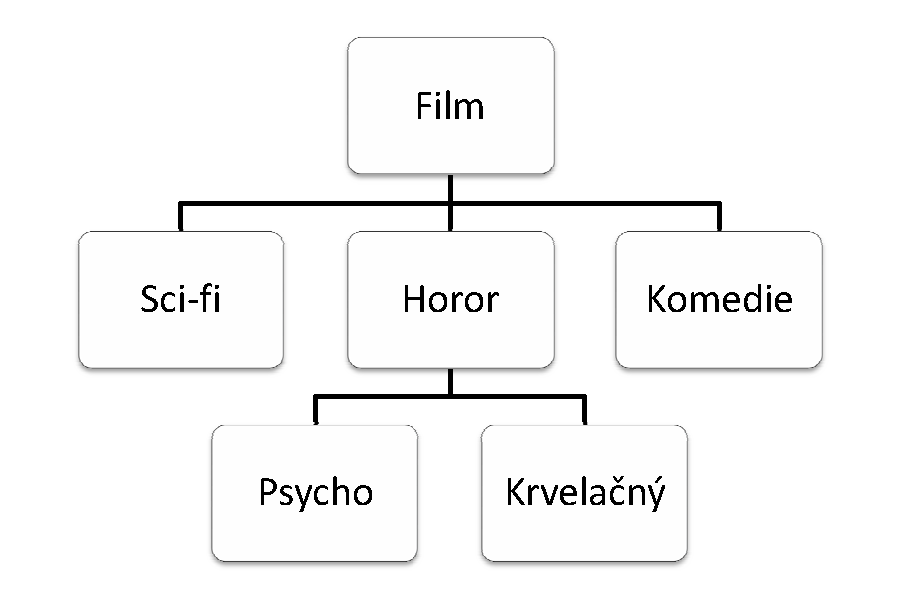
\includegraphics{figures/movieClasses}
\caption{Příklad hierarchie tříd v ontologii domény filmu.}
\label{img:movieClasses}
\end{center}
\end{figure}

\textit{Instance} odpovídá konkretnímu objektu reálného světa. Zda určitý objekt považovat za instanci či třídu není však čistě objektivní, závisí na konkrétním využití ontologie \cite{ontowww}.

\textit{Axiomy} jsou pravidla, které je možné do ontologie přidávat. Vyjadřují např. ekvivalenci a disjunkci tříd.

\section{Vytváření ontologie}

V této sekci si ukážeme, jak se taková ontologie připravuje.

\subsection{Ontologie vína}

Třídy utvářejí představu o doméně. Například třída vín reprezentuje všechna vína.
Konkrétní vína jsou instancemi tříd těchto vín, tedy např. Bordeaux víno je instancí třídy "Bordeaux vína".
Třídy mohou mít podtřídy, kde každá podtřída blíže specifikuje rodičovskou třídu.
V našem příkladu můžeme třídu všech vín rozdělit na podtřídy červené, bílé a růžové (nebo také na suché, polosuché, polosladké, sladké či na perlivé, šumivé, stolní...) \cite {noy}.

Atributy popisují vlastnosti tříd a instancí. Château Lafite Rothschild Pauillac je vyráběn v Château Lafite Rothschild vinici (viz obr. \ref{img:wine}).
Máme tedy atribut vína "výrobce" s hodnotou Château Lafite Rothschild vinice.
Na úrovni tříd můžeme říci, že instance třídy Víno budou mít atributy pro vyjádření příchuti, obsahu cukru, výrobce atp. 

Atributy "výrobce" všech instancí třídy Víno, včetně její podtřídy Pauillac, mají jako hodnotu instanci třídy Vinice (viz obr. \ref{img:wine}).
Všechny instance třídy Vinice mají vlastnost "vyrábí", která ukazuje na všechny vína (= instance třídy Víno a její podtřídy), která daná vinice vyrábí.

Vývoj ontologie obsahuje kroky:

\begin{itemize}
\item Definování třid ontologie.
\item Taxonomické uspořádání tříd (vytvoření hierarchie).
\item Definování atributů a jejich dovolených hodnot.
\item Naplnění instancí a atributů konkrétními hodnotami.
\end{itemize}

\begin{figure}[h]
\begin{center}
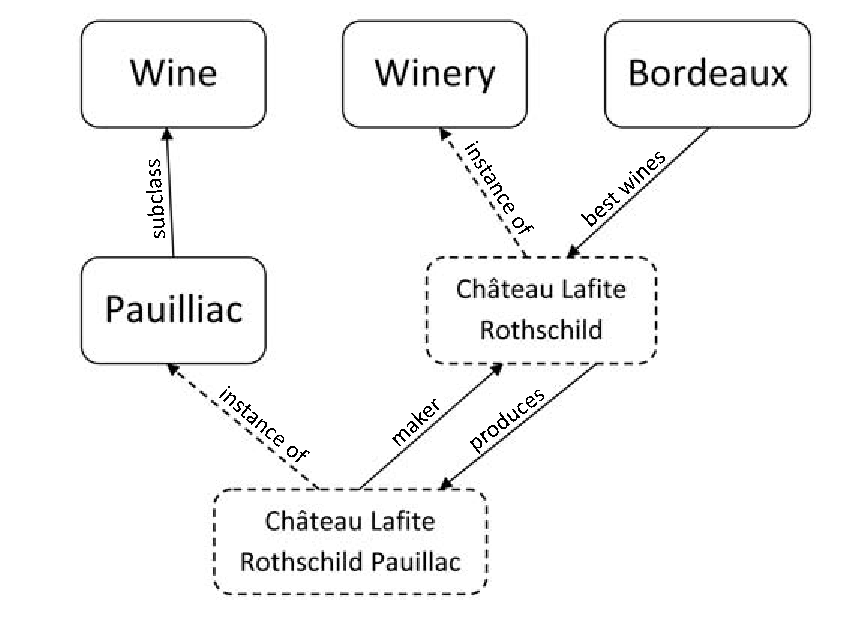
\includegraphics{figures/wine}
\caption{Ukázka ontologie vína resp. některých tříd a vazeb mezi nimi. Čárkované boxy představují instance, ostatní boxy značí třídy. Šipky značí jednotlivé vztahy.}
\label{img:wine}
\end{center}
\end{figure}

Další podrobnější příklad vytváření ontologie uvádí \cite{owltutorial} jako ontologii Pizzy \cite{pizza}.

\section{Jazyky ontologie}
\label{chapter:ontologyLanguage}

Každá ontologie, aby mohla být strojově čitelná, musí být zapsána formálně, pomocí jazyka. Takový jazyk se nazývá jazykem ontologie. 
Ontologické jazyky umožňují tvůrcům ontologií jednoznačně a formálně popsat konceptualizaci, tj. systém pojmů modelující určitou část světa. 
Hlavní požadavky na tyto jazyky jsou \cite{staab}:

\begin{itemize}
\item správně definovaná syntaxe
\item vhodná podpora dedukce 
\item formální sémantika
\item adekvátní výrazové schopnosti
\end{itemize}

Formální sémantika zajišťuje správně vyjádření znalostní struktury. Umožňuje různým lidem či zařízením stejnou interpretaci ontologie. 
Umožňuje na základě znalostí vyvozovat závěry. K tomu napomáhají i následující tvrzení \cite{staab}:
\begin{itemize}
\item Členství ve třídě - Jestliže x je instance třídy B a B je podtřídou třídy A, potom můžeme tvrdit, že x je instancí třídy A.
\item Ekvivalence tříd - Jestliže třída A je ekvivalentní s třídou B a třída B je ekvivalentní s třídou C, poto je třída A ekvivalentní s třídou C.
\item Konzistence tříd - Jestliže jsou dvě třídy disjunktní, podtřída obou těchto tříd bude prázdná.
\item Klasifikace tříd - Mějme definované vlastnosti třídy A, pak můžeme tvrdit: Pokud instance x má stejné vlastnosti, je tato instance x instancí třídy A.
\end{itemize}

Výrazová schopnost jazyka se volí podle účelu nasazení. Čím větší vyjadřovací schopnosti jazyk ale má, tím více se stává složitějším pro počítače.
Např. v jazyce OWL existují hned tři úrovně výrazovosti (OWL Lite, OWL DL, OWL Full). 
U jazyka OWL Full je už pro počítač mnohdy složité dopočítat se výsledku.

    \subsection{Resource Description Framework}
        
        Jedním z pilířů Sémantického webu je technologie Resource Description Framework (RDF) \cite{semWeb}, 
        jedná se o jazyk reprezentující informace o zdrojích ve webovém prostředí \cite{RDFprimer}, umožňuje výměnu a sdílení znalostí na webu \cite{RDF}.
        
        RDF nám umožňuje pracovat s informacemi na webu, namísto pouhého zobrazení dat uživateli. Díky RDF totiž počítač těmto datum rozumí, např. jméno osoby chápe jako skutečné jméno a ne jen jako pouhý shluk písmen. Jednotlivé aplikace tak mohou s informacemi pracovat a sdílet mezi sebou. 
        
        RDF je založeno na identifikaci všech věcí pomocí webových identifikátorů Uniform Resource Identifiers (URI). Popisuje informace jednoduše pomocí klíče:hodnoty, resp. vlastnosti a její hodnoty. Díky tomu může RDF jednoduše zobrazit informace jako graf uzlů a hran reprezentující zdrojová data \cite{RDFprimer}.
        
        Např. Eric Miller je jako osoba definována http://www.w3.org/People/EM/contact\#me, která má dále email a titul. RDF graf tohoto příkladu uvádí obr. \ref{img:miller}.
        
        \begin{figure}[h]
        \begin{center}
        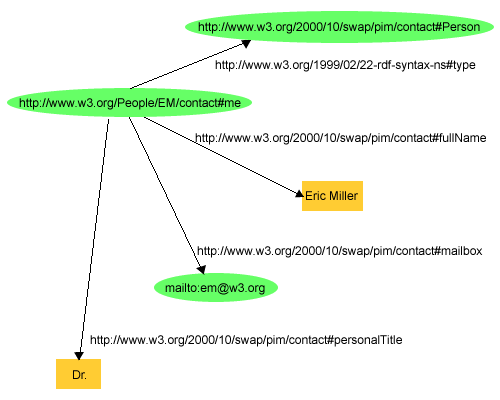
\includegraphics[width=11cm]{figures/rdf}
        \caption{RDF graf popisující osobu Eric Miller. (Zdroj \cite{RDFprimer})}
        \label{img:miller}
        \end{center}
        \end{figure}

        Další způsob reprezentace RDF je vedle grafu tzv. trojice. V troj-notaci je každý výrok zapsán jako trojice \textit{podmět, predikát, předmět} (v tomto pořadí). 
        Např. výrok "Osoba se jmenuje Eric Miller" z příkladu \ref{img:miller} se zapíše jako:
        
        \begin{verbatim}
        http://www.w3.org/People/EM/contact#me 
        http://www.w3.org/2000/10/swap/pim/contact#fullName 
        http://www.w3.org/2000/10/swap/pim/contact#mailbox
        \end{verbatim}
        Předchozí trojice by měla být zapsána do jednoho řádku, pro lepší přehlednost zde však uvádíme v řádcích.
        
        \subsubsection{Resource Description Framework in attributes} 
        \label{chapter:rdfa}
        
        Resource Description Framework in attributes (RDFa) je další W3C\footnote{World Wide Web Consortium (W3C) je hlavní standardizační organizace pro WWW.} specifikace.
        RDF je v praxi oddělený, samostatný soubor, sloužící jen pro webovou aplikaci, zatímco uživateli je nabídnuta XHTML stránka. 
        RDFa oproti tomu umožňuje vkládat RDF trojice přímo do XHTML dokumentů a tím tak podobně jako mikroformáty obohacují data o metadata \cite{RDFa}.
        
        \subsubsection{Resource Description Framework Schema}
        
        Resource Description Framework Schema (RDFs) je sémantickým rozšířením jazyka RDF.
        RDFs je nadstavbou RDF, doplňuje třídy a možnost stanovit definiční obor a obor hodnot. RDFs umožňuje zachycení sémantiky obsahu stránek \cite{ontowww}.
        
        \subsubsection{RDF/XML}
        
        RDF/XML je serializace RDF grafů do XML syntaxe \cite{rdfxml}. 
    
    \subsection{SPARQL Protocol and RDF Query Language}
    
    SPARQL Protocol and RDF Query Language (SPARQL) - název je rekurzivní zkratka - je další klíčovou technologií Sémantického webu \cite{sparqlwiki}.
    SPARQL je, jak vyplývá z názvu, dotazovací jazyk pro RDF. Vyhledává množiny trojic, které vyhovují zadanému dotazu.   
    Výsledkem SPARQL dotazu je opět trojice či množina trojicí podmět, predikát, předmět.
    
    Vzorový SPARQL dotaz:
    
    \begin{verbatim}
    PREFIX abc: <http://example.com/exampleOntology#> 
    SELECT ?capital ?country
    WHERE {
      ?x abc:cityname ?capital ;
         abc:isCapitalOf ?y .
      ?y abc:countryname ?country ;
         abc:isInContinent abc:Africa .
    }
    \end{verbatim}
    
    vrátí množinu trojic:
    
    \begin{verbatim}
    ?capital http://example.com/exampleOntology\#isCapitalOf ?country
     \end{verbatim}
     
     Jinými slovy vráti seznam všech zemí a jejich hlavních měst v Africe.
        
    \subsection{Ontology Web Language}

    Ontology Web Language (OWL) vznikl pod záštitou W3C a vychází z DAML+OIL ontologického jazyka \cite{owlguide}.
    Je dalším jazykem pro vytváření ontologií a rozšiřuje vyjadřovací schopnosti jazyka RDF resp. přidává mu další sémantickou vrstvu. \cite{semWebStandards}.
    Má např. bohatší sadu operátorů (and, or, negace) \cite{owltutorial}a zavádí disjunktní třídy a kardinalitu vztahu \cite{staab}. 
    Vyjadřovací schopnosti naznačuje obrázek \ref{img:owlexpressiveness}
    
    \begin{figure}[h]
    \begin{center}
    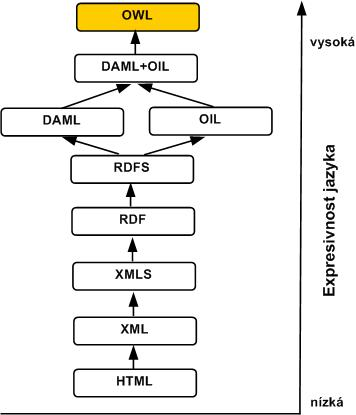
\includegraphics[width=8cm]{figures/owlexpressiveness}
    \caption{Vyjádření expresivnosti OWL jazyka. (Zdroj \cite{owlhradec})}
    \label{img:owlexpressiveness}
    \end{center}
    \end{figure}
        
        \subsubsection{Dialekty OWL}
        
            OWL ontologie byly vyvinuty ve třech verzích (syntaktických podmnožinách), a to OWL-Lite, OWL-DL a OWL-Full lišící se svoji vyjadřovací schopností \cite{owlguide}:
            
            \begin{itemize}
            \item \textbf{OWL Lite} má nejmenší vyjadřovací schopnosti. 
            Je navržen pro použití v situacích, kde stačí jednoduchá hiearchie tříd a jsou požadovány jen jednoduché omezení (např. kardinalita pouze 0 či 1).
            
            \item \textbf{OWL DL} nabízí vysokou míru vyjadřovacích schopností s garancí vypočítatelnosti (vždy se lze dobrat výsledku v konečném čase). 
            OWL DL je založena na deskripční logice (odtud zkratka DL). 
            Deskripční logika vychází z predikátové logiky, je ale omezenější \cite{svatek}.
            
            \item \textbf{OWL Full} obsahuje kompletní vyjadřovací sílu a plnou syntaxi RDF Schema, díky čemuž ale není garantována vypočítatelnost (dobrání se výsledku). 
            \end{itemize}
            
            Každý z výše popsaných podjazyků je rozšířením svého jednoduššího předchůdce, tzn. každá syntakticky správná OWL Lite ontologie je zároveň správnou OWL DL ontologií a každá správná OWL DL ontologie je OWL Full ontologií.
            Stejný princip platí i u vyvozování těchto ontologií.
            
        \subsubsection{Komponenty OWL}
            
            Mezi základní kompomenty OWL jazyka patří \cite{owltutorial}:
            
            \begin{itemize}
            \item \textbf{Individua (instance)} - Individua reprezentují skutečné objekty v rámci domény, kterou se zabýváme. Jedná se o instance tříd.
            Příklad znázornění instancí ukazuje obrázek \ref{img:individuals}.
            
            \begin{figure}[h]
            \begin{center}
            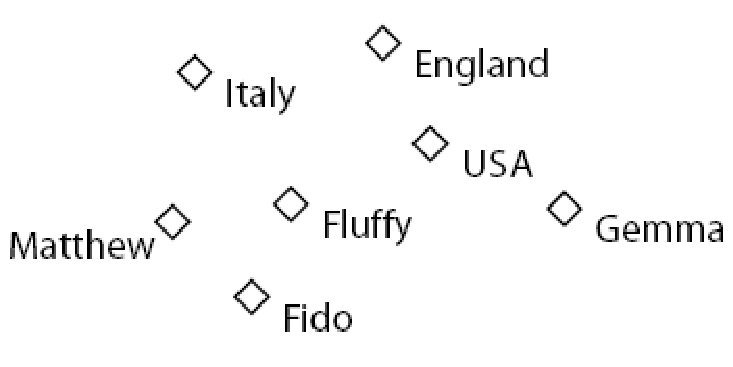
\includegraphics[width=10cm]{figures/individuals}
            \caption{Příklad instancí. (Zdroj \cite{owltutorial})}
            \label{img:individuals}
            \end{center}
            \end{figure}
            
            \item \textbf{Vlastnosti} - Vlastnosti se používají k definici vztahu mezi dvěma objekty (individui). Mohou mít inverze, mohou bít funkční (tj. mohou mít pouze jednu hodnotu), tranzitivní\footnote{Mějmě vlastnost T a instance a,b,c. Vlastnost T je tranzitivní, jestliže a T b a zároveň b T c, potom platí i a T c. Zdroj \cite{relace}} a symetrické\footnote{Mějme vlastnost S a instance a,b. Vlastnost S je symetrická, pokud platí a S b a zároveň b S a. Zdroj \cite{relace}}.
            Obrázek \ref{img:properties} představuje instance a jejich vztahy (vlastnosti).
            
            \begin{figure}[h]
            \begin{center}
            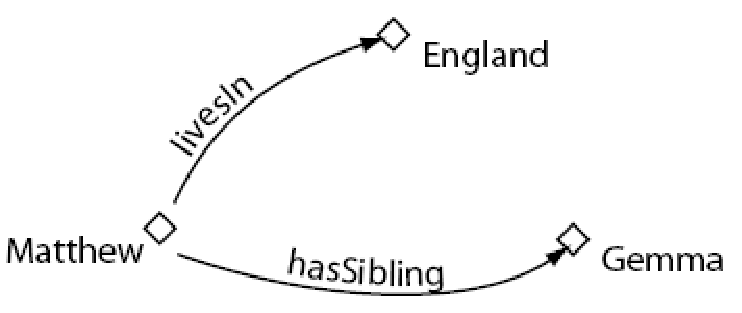
\includegraphics[width=10cm]{figures/relations}
            \caption{Příklad vztahů mezi individui. (Zdroj \cite{owltutorial})}
            \label{img:properties}
            \end{center}
            \end{figure}
            
            
            \item \textbf{Třidy} - Můžeme si je představit jako množiny obsahující individua, které spolu sdílejí některou vlastnost.
            Obrázek \ref{img:classesindividuals} vyjadřuje několik tříd obsahující instance (kde některé instance mají mezi sebou vztah). 
            
            \begin{figure}[h]
            \begin{center}
            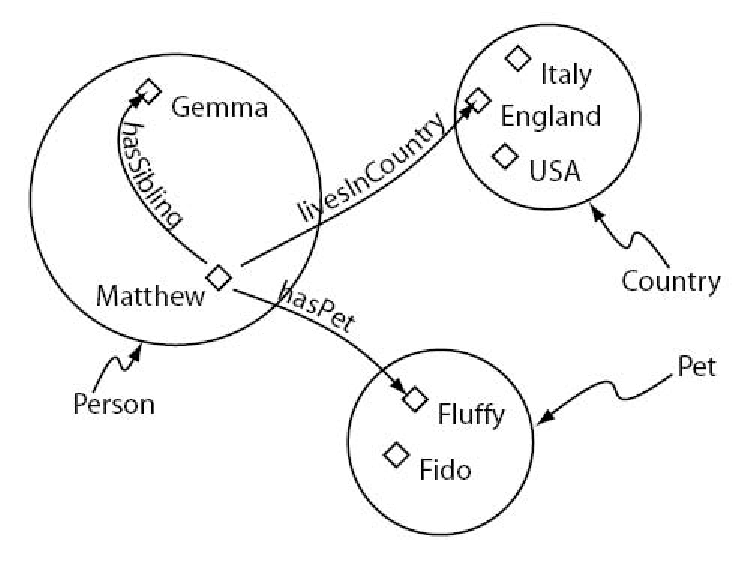
\includegraphics[width=10cm]{figures/classes}
            \caption{Příklad tříd s instancemi. (Zdroj \cite{owltutorial})}
            \label{img:classesindividuals}
            \end{center}
            \end{figure}
            
            \end{itemize}
            
        \subsubsection{OWL 2}  
            
        OWL2 je ontologický jazyk Sémantického webu, který schválila skupina W3C jako své doporučení v říjnu 2009. Nahrazuje a rozšiřuje původní OWL jazyk z roku 2004 (zpětně označovaného jako OWL 1), se kterým je zpětně kompatibilní. Jazyk je stále založen na RDF a původní OWL 1 doplňuje např. o klíče, řetezení vztahů, bohatší datové typy, dále přidává možnost asymetrických a disjunktních vztahů.
        Obrázek \ref{img:owl2} ukazuje základní stavební bloky a jejich propojení. Elipsa představuje abstraktní notaci ontologie (může být buď jako abstraktní struktura či jako RDF graf). Nahoře jsou konkrétní varianty syntaxe, které OWL 2 může používat k serializaci ontologie. Dole pak jsou dvě sémantické specifikace definující význam OWL 2 ontologií.
        Jako hlavní serializaci OWL 2 používá RDF/OWL \cite{owl2}.
       
        \vspace*{6pt}
        \textbf{Dialekty a Profily OWL 2}
        \vspace*{6pt}
       
        OWL 2 definuje dva podjazyky OWL 2 DL a OWL 2 Full.
        Dále definuje OWL 2 Profily jako podjazyky (syntaktické podmnožiny) jazyka OWL 2. Jsou definovány tři profily: OWL 2 EL, OWL 2 QL a OWL 2 RL definované opět jako syntaktické podmnožiny OWL 2. Každý z profilů je více restriktivní než jazyk OWL 2 DL \cite{owl2primer}. 
        
        OWL 2 Profily \cite{owl2primer}:
        
        \begin{itemize}
        \item \textbf{OWL 2 EL} je podobný OWL 2 DL s některými omezeními. Zkratka EL značí tzv. EL deskripční logiku\footnote{EL je malá deskripční logika \cite{EL}}.
        
        \item \textbf{OWL 2 QL} může být realizován použitím standartních relačních databázových technologií jako je např. Structured Query Language (SQL). Díky tomu může být pevně sloučen s Relational database management system (RDBMS). Zkratka QL tedy značí Query Language.
        
        \item \textbf{OWL 2 RL} je určen pro aplikace vyžadující různou škálu logického usuzování (reasoning) bez přílišného obětování vyjadřovací síly.
        \end{itemize}
        
        \subsubsection{OWL/XML}
        
        Obdobně jako RDF/XML je OWL/XML serializací OWL ontologie do XML syntaxe \cite{owlxml}.
        
\section{Analýza nástrojů na tvorbu ontologií}

\subsection{Editor ontologií}
Pro navrhování a modelování ontologií potřebujeme vhodný nástroj pro editaci ontologií, težko budeme ontologii vytvářet čistě v textovém editoru (teoreticky to však samozřejmě při dobré znalosti konkrétní syntaxe lze).

Nejpoužívanějším editorem ontologií je \textit{Protégé}\footnote{Protégé \url{http://protege.stanford.edu/} vyvíjený v rámci projektu CO-ODE \url{http://www.co-ode.org/}.}, vytvořený na Standford University jako open-source \cite{owl2primer}.
Díky jeho otevřené formě lze do Protégé doplňovat nejrůznější zásuvné moduly (za všechny např. plugin OWL Wiz vizuálně znázorňující strukturu ontologie).
Protégé umožňuje exportovat vymodelovanou ontologii do různých syntaxí (např. RDF/XML, OWL/XML, OWL functional, Manchester OWL, turtle).

Dalším open-source nástrojem je \textit{SWOOP}\footnote{SWOOP \url{http://code.google.com/p/swoop/}} podobný Protégé. Dovede např. přehledně zobrazit syntaxi jen pro vybrané prvky ontologie, a to současně v abstraktní syntaxi, RDF/XML a Turtle syntaxi.

Poslední zmíním velmi povedený editor \textit{NeOn Toolkit}\footnote{NeOn Toolkit \url{http://www.neon-toolkit.org/}} postavený na Eclipse platformě, který také umožňuje přidání velkého množství zásuvných modulů.

K vytvoření hudební ontologie pro tuto práci budeme používat editor Protégé 4.0, a to z důvodu jeho rozšířenosti, podpoře exportu do různých syntaxí a vizualizačního pluginu.

\subsection{Programovací prostředí}

S vymodelovanou ontologií chceme dále pracovat, použít ji ve vhodné aplikaci, proto musíme v závislosti na programovacím jazyku zvolit vhodný nástoj, který mám s implementací pomůže. 
Naštěstí pro tyto účely dnes existuje spousta nástrojů \cite{semwebtools}.

Pro programovací jazyk Java je zřejmě nejrozšířenější nástroj \textbf{Jena Semantic Web Framework}\footnote{Jena Semantic Web Framework \url{http://jena.sourceforge.net/}}, který poskytuje programovací prostedí pro RDF, RDFS, OWL a SPARQL.

Pro PHP: Hypertext Preprocessor (PHP) prostředí existují tři hlavní nástroje, ARC, RAP, a Triplify \cite{semwebwikitools}:

\begin{itemize}
\item \textbf{ARC}\footnote{ARC \url{http://arc.semsol.org/}} (resp. ARC2) je open-source flexibilní RDF systém pro sémantický web postavení na PHP. Obsahuje několik RDF parserů (RDF/XML, Turtle, RSS, mikroformáty, RDFa atd.) a serialuzuje např. do RDF/JSON, RDF/XML a Turte. ARC dále pracuje se SPARQL dotazovacím jazykem. 
S RDF daty pracuje přes RDF Store pomocí MySQL databáze. 
RDF Store je systém pro ukládání a správu RDF dat \cite{rdfstore}. 

\item \textbf{RAP}\footnote{RAP \url{http://www.seasr.org/wp-content/plugins/meandre/rdfapi-php/doc/index.html}} je RDF API pro PHP. RAP je systém pro parsování, dotazování, manipulaci, serializaci a obsluhu RDF. 

\item \textbf{Triplify}\footnote{Triplify \url{http://triplify.org/}} je plugin pro webové aplikace, který relační databázi transformuje do RDF či do JavaScript Object Notation (JSON) podoby a z databáze tak díky tomu vytváří sémantickou strukturu.
\end{itemize}

Seznam dalších nástrojů i pro jiné programovací jazyky (jako např. Python, C, C++, C\#, Perl, Ruby, Flex atd.) nabízí \cite{semwebtools}.

Pro tento projekt použijeme ARC systém (důvody proč právě ARC uvádím v následující kapitole \ref{chapter:webappdesign}).  

%*****************************************************************************
\chapter{Analýza a návrh řešení}

\section{Představa aplikace}
\label{chapter:requirements}

Navržená ontologie hudby by pro naše účely hudebního přehrávače měla popisovat hudbu takovým způsobem, aby pokryla požadavky a očekávání uživatele hudebního přehrávače.


Potenciální posluchač, než začne samotnou hudbu poslouchat, potřebuje napřed požadovanou hudbu nalézt (ať již na svém kapesním přehrávači či ve webové aplikaci).
Nejjednodušší cesta k nalezení konkrétní hudby samozřejmě nastává v situaci, kdy uživatel přesně ví, jaký název písně či interpreta požaduje. Uživatel si ale pouze s tímto základním vyhledáváním nevystačí.
Uživatel může mít např. chuť poslouchat jeho oblíbený žánr a nezáleží mu na konkrétním interpretovi. 

Nebo naopak. V běžném životě si člověk zcela přirozeně řekne, že se mu líbí určitý hudební interpret, a že by rád poslouchal jemu podobnou hudbu. Proto stejně tak přirozené by mělo být tuto myšlenku převést do hudebního přehrávače.
Převeďme si tuto myšlenku do věty v přirozeném jazyce, tedy např. "Líbí se mi hudba Michaela Jacksona". 
Pokud vám někdo tuto větu řekne a zároveň vás požádá, abyste mu sdělili podobnou hudbu, jste schopni mu odpovědět, a to na základě znalostí, které máte či které si dohledáte.
 
Stejnou komunikaci mezi lidmi se tedy pokusíme převést do počítačové podoby. 
Dotázaný člověk v našem příkladu, jak již bylo řečeno, odpovídal na základě \textit{znalostí}. Bez potřebných znalostí by totiž nemohl tazateli odpovědět.
Pro úspěšné převedení takové komunikace tedy evidentně musíme počítači zajistit potřebné znalosti, aby i on věděl stejně jako vědí lidé, že Michaelu Jacksonovi je podobná např. Whitney Houston s Madonnou, zatímco např. takový Marilyn Manson s ním nemá nic společného. 

Ideálním nástrojem pro počítač, aby mohl odvozovat takovéto vzájemné vztahy, je zcela jistě ontologie.
Pomocí ontologie totiž můžeme vyrobit potřebnou znalostní bázi, z které pak náš program bude čerpat a na jejím základě může vyhodnocovat potřebné znalosti a ve výsledku tak nabízet pro uživatele relevantní informace.

Další možností, kterou se tato práce dále nezabývá, vyhledávání příbuzné hudby je cestou přes porovnávání zvukového signálu.

Uživatel může mít dále touhu poslouchat směsici různých žánrů. Má chuť např. na britský pop říznutý Rock\&Rollem.
Nebo je uživatel dokonce milovník a znalec konkrétních hudebních nástrojů či by si jen rád poslechl nějakou kvalitní elektrickou kytaru.

Všechny výše zmíněné požadavky se v práci pokusíme uspokojit formou webové aplikace.

\section{Současná řešení}

    Podívejme se nyní na současný stav souvisejících řešení.
    
    Se základním relačním databázovým modelem pro popis hudby přišly projekty \textit{FreeDB} \cite{freedb} a \textit{MusicBrainz} \cite{musicbrainz}.
    Tyto dvě služby nabízejí velkou databázi hudebních interpretů, jejich děl apod. Dále zmiňme např. projekt DBpedia, který se úspěšně snaží transformovat data z Wikipedie do strukturovanější, sémantičtější podoby \cite{dbpedia}. 
    
    V r. 2004 vznikla služba MusicBrainz Metadata Vocabulary \cite{musicbrainzmetadatavoc}, která využila databázi MusicBrainz a vytvořila z ní ontologii. Tehdy ještě ale MusicBrainz nebyl vyvinut natolik jako dnes.
    Novější a známější projekt \textit{Music Ontology}, který vymyslel Frédérick Giasson, opět čerpá z MusicBrainz databáze a vytváří novou hudební ontologii využívající W3C RDF technologii \cite{mo}. 
    Music Ontology tedy ve výsledku umožňuje SPARQL dotazování nad MusicBrainz databází, a to právě díky RDF, ve kterém je ontologie napsána (resp. samotná ontologie je vyjádřená pomocí RDF/XML).
    
    Navíc Music Ontology využívá dalších praktických ontologií, jako je \textit{The Friend of a Friend (FOAF) project}, který umožňuje sdílení a propojení informací o lidech, místech a dalších věcech, které jsou dostupné na webu \cite{foaf}.
    Music Ontology dále používá \textit{Event Ontology}, kterou používá k popisu různých událostí (např. koncerty a vystoupení, nahrávky) \cite{event} současně s \textit{Timeline Ontology} popisující informace z hlediska času \cite{timeline}.

    Praktickým vyústěním Music Ontology jsou např. aplikace Pandora\footnote{Pandora \url{http://www.pandora.com/}}, velmi populární služba last.fm\footnote{last.fm \url{http://www.last.fm/}} a zřejmě nejčerstvější BBC Music\footnote{BBC Music \url{http://www.bbc.co.uk/music}}.

\section{Návrh hudební ontologie}

Naší snahou je vymodelovat vlastní hudební ontologii za vhodného použití FOAF příp. Event/Timeline ontologie.

Ontologii budeme vyvíjet v editoru Protégé 4.0 a výsledek budeme ukládat do formátu RDF/XML, jelikož je tento druh serializace nejběžněji používaný. RDF/XML formát používá mimo jiné právě i již zmíněná Music Ontology a jazyk OWL 2 jej vyžaduje jako primární syntaxi (což je videt např. z obr. \ref{img:owl2}).

Volně se necháme inspirovat projektem Music Ontology, nicméně se pokusíme hudební ontologii postavit sami dle svého nejlepšího uvážení. 
Výslednou ontologii pak můžeme s Music Ontology porovnat.

Při vytvoření ontologie v Protégé tedy naimportujeme FOAF a Event ontologii (předpokládáme jejich využití) a začínáme modelovat vlastní hudební ontologii.

Zvykem je začínat od třídy \textit{Thing}, tedy "věc", která zastřešuje všechny další třídy. Lépe se nám pak uvažuje hierarchie, lépe si ji dovedeme představit - pokud by tato třída neexistovala, všechny její podtřídy by chaoticky "létaly" ve vzduchu. Její existence nám pomáhá ke klasické stromové struktuře, na kterou jsme navyklí (viz obr. \ref{img:thing2}). Stejný obrázek dále ukazuje, které třídy jsme v naší ontologii nějakým způsobem použili (samozřejmě některé mají další podtřídy, na obrázku nezobrazené).

\begin{figure}[h]
\begin{center}
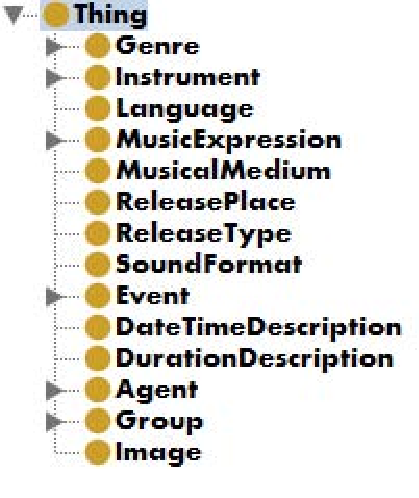
\includegraphics[width=5cm]{figures/thing2}
\caption{Nadtřída Thing obsahující všechny použité třídy}
\label{img:thing2}
\end{center}
\end{figure}

Třídy a podtřídy jsou mezi sebou definované vztahem "IS-A", tedy každá potřída rozšiřuje vlastnosti svého rodiče. Vztah mezi třídy znázorňuje obrázek \ref{img:thing}

\begin{figure}[h]
\begin{center}
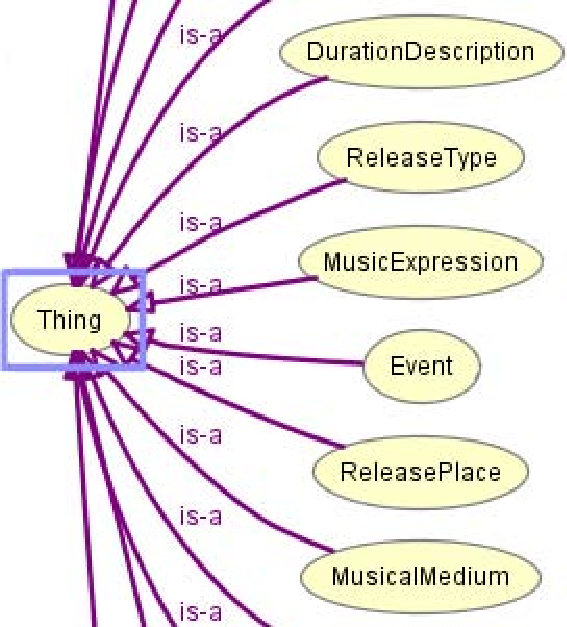
\includegraphics[width=6.5cm]{figures/thing}
\caption{Ukázka "IS-A" vztahu mezi třídou-podtřídou}
\label{img:thing}
\end{center}
\end{figure}

Hierarchii tříd jsme modelovali podle našeho uvážení tak, aby vyhovovala našemu účelu. 

Ontologii Event jsme použili na třídu Event, ve které jsou podtřídy definující konkrétní typ události (viz obr. \ref{img:event}).

\begin{figure}[h]
\begin{center}
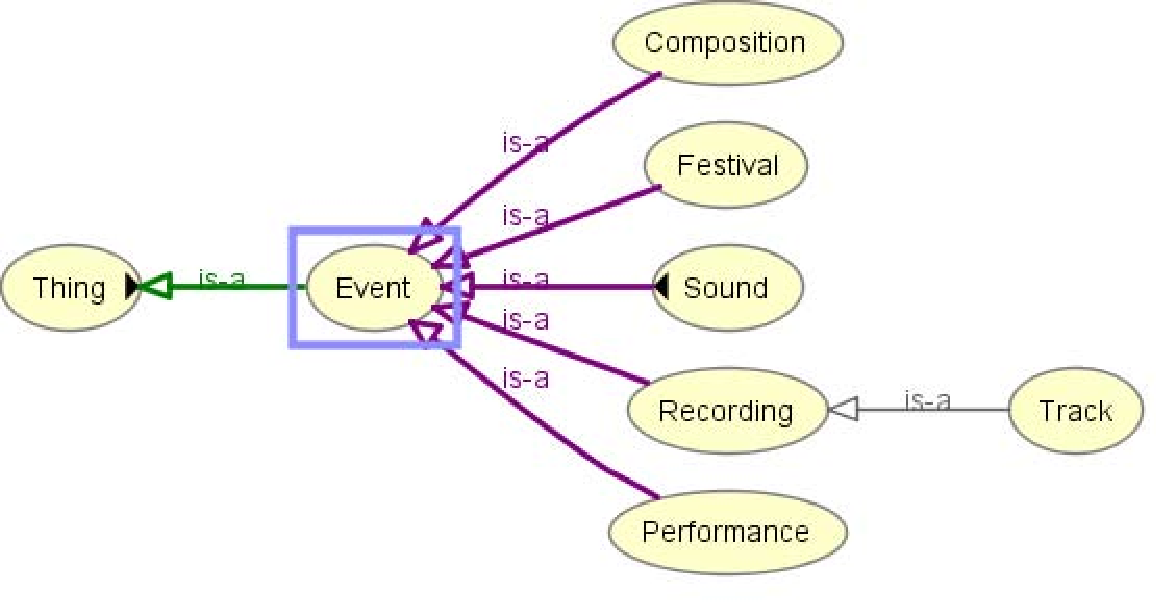
\includegraphics[width=13cm]{figures/event}
\caption{Třída Event patřící do importované Event Ontology a její rozšíření v rámci naší ontologie}
\label{img:event}
\end{center}
\end{figure}

Třídy Agent, Person, Group a další jsou definované přes importovanou ontologii FOAF (viz obr.\ref{img:foafclasses}).
V návrhu ontologie jsme využili i vztahy definované FOAF ontologií. Např. jména instancím či přiřazení člena do určité kapely jsme přidávali přes FOAF vlastnosti foaf:name či foaf:member.

Význam FOAF a Event vztahů a tříd je dán definicí podle těchto ontologií a tím je zajištěna jejich srozumitelnost např. při sdílení ontologie na webu. 

\begin{figure}[h]
\begin{center}
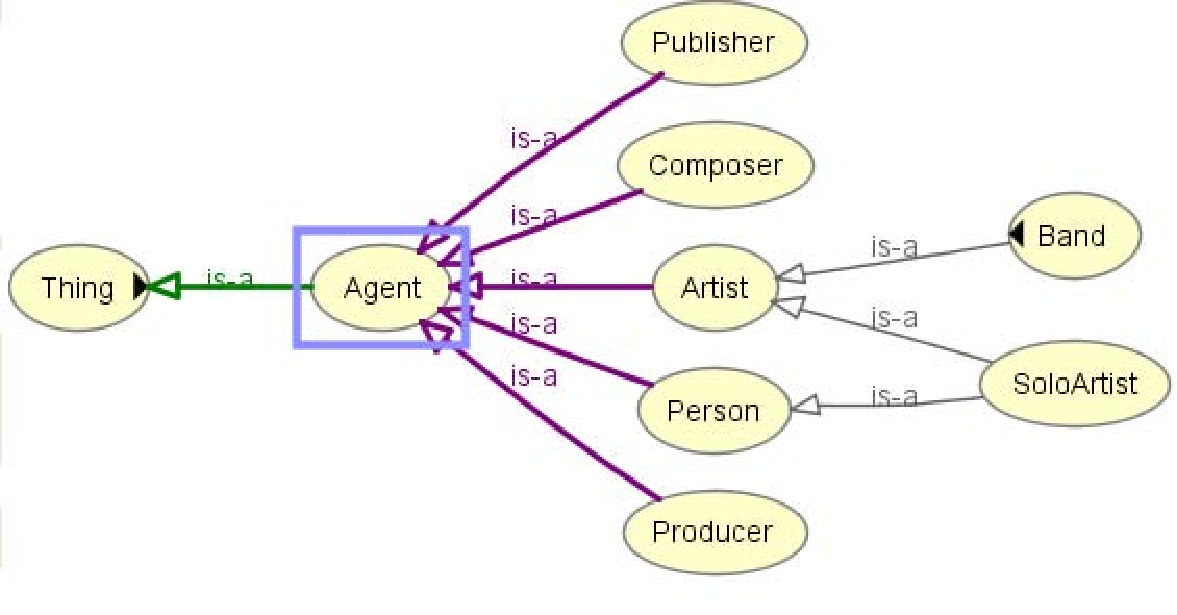
\includegraphics[width=13cm]{figures/foafclasses}
\caption{Ukázka třídy Agent a jejích podtříd. Agent a Person jsou definovány z FOAF ontologie a tím je zajištěn jejich patřičný význam.}
\label{img:foafclasses}
\end{center}
\end{figure}

Výsledná struktura tříd navržené ontologie je zobrazena na obrázku \ref{img:ontoFinal}. 
Z úsporných důvodu jsou však hudební nástroje a žánry zobrazeny zvlášť. 

Pro hudební nástroje jsem vytvořil hiearchii tříd podle celosvětově uznávané hudební klasifikace Hornbostel-Sachs \cite{hornsachs}.
Tím naší ontologii vdechneme potenciál pro možné využití mezi hudebně odbornou veřejností. Částečné (z úsporných důvodů) schéma hudebních nástrojů je vyobrazeno na obrázku \ref{img:ontoFinalInstruments}. Celá struktura hudebních nástrojů je dostupná na stránkách projektu.

Struktura hudebních žánrů byla vytvořena více či méně podle \cite{allmusic} a výsledek naleznete na obr. \ref{img:ontoFinalGenres}.

\textbf{Pozn.}: Všechny schémata použité v této části kapitoly zobrazující strukturu tříd jsou zobrazením pouze tříd, nikoliv instancí.

Plnou dokumentaci hudební ontologie vytvořenou přes OWLDoc plugin\footnote{OWLDoc plugin do Protégé \url{http://www.co-ode.org/downloads/owldoc/}} naleznete na webových stránkách projektu\footnote{Stránky projektu \url{http://martindoubravsky.cz/ctu/}}.

Výslednou hudební ontologii včetně naplněných testovacích instancí si je možné prohlížet taktéž online pomocí aplikace \textit{Ontology Browser} vytvořené projektem CO-ODE \footnote{Ontology Browser \url{http://code.google.com/p/ontology-browser/}}.

\section{Návrh webové aplikace}
\label{chapter:webappdesign}

Pro vytvořenou ontologii navrhneme webovou aplikaci, která bude umožňovat uživateli v ontologii vyhledávat podle požadavků sepsaných v kapitole \ref{chapter:requirements}.

Pro webové prostředí použiji programovací jazyk PHP, a to z důvodu, že je mi tento jazyk bližší než např. Java, ve které by aplikace postavit samozřejmě šla také.
Dále volím PHP z důvodu možného budoucího srovnání jazyků PHP a Java, jak si vedou při zpracovávání ontologií (v současné době vyvíjí kolega jiný projekt postavený také na ontologii a právě na Javě, výsledky proto bude možné porovnat).

Pro práci s ontologií jsem na základě analýzy zvolil systém ARC, což je RDF systém pro sémantický web běžící na PHP.
ARC je zdarma jako open-source, je snadno použitelný a umožňuje dotazovat se přímo pomocí SPARQL dotazů.

Při vývoji webové aplikace budeme dbát na to, aby zůstala oddělena aplikační vrstva od vrstvy prezentační. 

Výstup aplikace bude formou webové stránky v jazyce HTML 5, což je nová stále se ještě vyvíjející verze jazyka HTML, přinášející podstatné změny a novinky (často kontroverzní). 

Vyhledávání v ontologii provedeme přes SPARQL výrazy vhodně zakomponované do PHP a ARC struktury.
Zřejmě přes HTML formulář vyplněný uživatelem odešleme hledaný výraz přes Hypertext Transfer Protocol (HTTP) a metodu GET. V PHP aplikační části tento hledaný výraz odbavíme a předáme systému ARC, který nad výrazem provede SPARQL dotazy a vrátí výsledek.
Výsledek uživateli zobrazíme přes jednoduché a použitelné grafické rozhraní.

%*****************************************************************************
\chapter{Realizace}
\label{chapter:implementation}

V této kapitole postupně vytvoříme výslednou webovou aplikaci.

\section{Použité technologie}

\subsection{Aplikační část}

\subsubsection{PHP}

Celá webová aplikace běží na PHP. Webhostingový server, na kterém je projekt umístěn, v současné době nabízí PHP verze 5.1.2, což je pro naše účely zatím dostačující. 

\subsubsection{ARC}

Pro parsování ontologie je použit ARC RDF systém verze 2. ARC si potřebné informace interně ukládá do MySQL databáze.

\subsubsection{SPARQL}

Pro dotazování nad ontologií ARC systém umožňuje přímo použití SPARQL dotazovacího jazyku.


\subsection{Prezentační část}

\subsubsection{HTML}

Prezentační část je nakódována v jazyce HTML 5.

\subsubsection{CSS}

Dále je prezentační část ostylována pomocí Cascading Style Sheets (CSS) využívající některé prvky z CSS 3.

\subsubsection{jQuery 1.3.2}

Pro vylepšení uživatelského rozhraní je použit JavaScript v podobě knihovny jQuery v1.3.2.


\section{Vývojové prostředí}

Aplikace byla vyvíjena na lokálním APACHE serveru umožňující PHP i MySQL. Server byl nainstalován pomocí XAMPP nástroje\footnote{XAMPP \url{http://www.apachefriends.org/en/xampp.html}} ve verzi 1.7.2, který je k dispozici zdarma a který všechny potřebné technologie (APACHE, PHP i MySQL) nainstaluje na náš lokální počítač.

Samotné zdrojové kódy aplikace byly napsány v textovém editoru PSPad 4.5.3\footnote{PSPad \url{http://www.pspad.com/}}, který je rověž zdarma.


\section{Vytvoření PHP aplikace}

Pro rozsáhlejší webovou aplikaci je velmi vhodné použít některý z dostupných PHP frameworků, který je založen na konceptu Model-View-Controller (MVC) oddělující jednotlivé vrstvy od sebe.
Pro naší aplikaci menšího rozsahu se ale nasazení frameworku nevyplatí, jelikož by samotný framework zabíral většinu aplikace a jeho vlastnosti by byly využity jen zcela minimálně.
Frameworky jsou výborná věc, to však neznamená, že je budeme slepě využívat kde nás napadne. Pro naší aplikaci by nasazení frameworku bohužel přineslo více práce než užitku.

Jednu věc ale z PHP frameworku alespoň částečně převezmeme, a to adresářovou strukturu Nette Frameworku \cite{nette}.
Začneme tedy vytvořím adresářové struktury našeho projektu, kterou navrhneme tak, abychom oddělili aplikační a prezentační vrstvu:

\begin{itemize}
\item[$\bullet$] app/ - obsahuje všechny soubory serverové části aplikace
    \begin{itemize}
    \item[$\bullet$] template/ - zde budou html šablony
    \item[$\bullet$] sparql/ - adresář pro zpracování sparql dotazů
    \item[$\circ$] bootstrap.php - zaváděcí soubor
    \end{itemize}
\item[$\bullet$] document\_root/ - adresář dostupný přes prohlížeč
    \begin{itemize}
    \item[$\bullet$] css/
    \item[$\bullet$] img/
    \item[$\bullet$] js/
    \end{itemize}
\item libs/ - knihovny
    \begin{itemize}
    \item[$\bullet$] ARC/
    \end{itemize}
\item[$\circ$] index.php - spouštění aplikace
\end{itemize}

V adresáři \verb|document_root/| jsou umístěny všechny kaskádové styly, obrázky a javascriptové soubory

Velmi důležité z hlediska bezpečnosti je zajistit, aby adresáře obsahující aplikaci a knihovny nebyly přístupné z webového prohlížeče.
Toho docílíme např. pomocí pravidel v souboru \verb|.htaccess|.

Soubor \verb|index.php| definuje cesty k dalším adresářům a předává řízení zaváděcímu souboru aplikace:

\begin{verbatim}
// absolute filesystem path to the web root
define('WWW_DIR', dirname(__FILE__) . '/document_root');

// absolute filesystem path to the application root
define('APP_DIR', WWW_DIR . '/../app/');

// absolute filesystem path to the templates 
define('TEMPLATE_DIR', APP_DIR . '/templates/');

// absolute filesystem path to the sparql queries
define('SPARQL_DIR', APP_DIR . '/sparql/');

// absolute filesystem path to the libraries
define('LIBS_DIR', WWW_DIR . '/../libs');

// load bootstrap file
require APP_DIR . '/bootstrap.php';
\end{verbatim}

V zaváděcím souboru \verb|bootstrap.php| nainstalujeme ARC systém, odbavíme dotaz zadaný uživatelem a předáme jej dále ke zpracování a definujeme šablonu, do které se má výstup vypsat.

Dále vytvoříme soubor \verb|query.php| ve kterém budeme rozhodovat, jakou část aplikace chce uživatel použít resp. v souboru zavoláme adekvátní soubor obsahující sadu SPARQL dotazů.
Stejně tak vytvoříme základní šablonu \verb|base.phtml|, která obsahuje prezentační html kód a do které vložíme šablonu odpovídající zpracovávané části aplikace. 


Nyní máme postavenou základní strukturu aplikace a můžeme se pustit do nastavení ARC systému.


\section{ARC systém}

Celý ARC systém nainstalujeme a nastavíme podle dokumentace dostupné na \cite{arc}.
Umístíme jej do adresáře \verb|libs| určeného pro knihovny.

V zaváděcím souboru systém nainstalujeme vyžádáním ARC konfigurační souboru \verb|config.php|, který zařídí načtení celé knihovny a zřídí přístup do databáze. 
Zde je potřeba zřídit systému přístup do databáze a správně nastavit přístupové údaje. Načtení knihovny se provede příkazem:

\begin{verbatim}
include_once LIBS_DIR . '/arc/ARC2.php';
\end{verbatim}

Specifické pro naší aplikaci je instalace ARC systému a následné načtení ontologie, které provedeme příkazem:

\begin{verbatim}
$store->query("LOAD <http://martindoubravsky.cz/ctu/mpo.owl>"); 
\end{verbatim}

Načtení ontologie provedeme při prvním spuštění aplikace nebo při provádění aktualizace ontologie. Nemá význam vynucovat načítání ontologie pokaždé, jelikož ARC systém si vše potřebné po načtení ontologie uloží do MySQL databáze, nad kterou pak vykonává SPARQL dotazy.
Navíc znovunačítání ontologie po určitou dobu zatěžuje server, proto je lepší při běžném provozu aplikace tento řádek kódu zakomentovat.

ARC systém obsahuje i soubor \verb|cli.php|, který slouží pro práci s PHP z příkazového řádku. Toho jsem využíval zejména při častých úpravách ontologie, kde sem mohl z příkazového řádku ontologii jednoduše v aplikaci aktualizovat. 

ARC systém je tedy naistalován a připraven k použití. Můžeme tedy přejít k nejdůležitější části aplikace a to k vlastnímu dotazování. 

\section{SPARQL dotazování}

Před vymýšlením samotných dotazů si musíme ujasnit, co chceme vyhledávat a jak toho chceme dosáhnout. Požadavky na vyhledávání jsou zmíněny v kapitole \ref{chapter:funcrequirements}.
Zbýva tedy určit způsob, jakým dosáhneme správných výsledků. 

V připraveném adresáři vytvoříme jednotlivé soubory odpovídající každý jednomu požadavku na hledání.
Soubor \verb|interpret.php| se bude zabývat vyhledáváním podobných interpretů,
soubor \verb|genre.php| bude prohledávat ontologii podle žánrů,
\verb|instrument.php| nabídne uživateli hledaní podle hudebních nástrojů a 
\verb|song.php| zpracuje požadavek na písně či alba.
Analogicky vytvoříme obdobnou strukturu šablon.

Nyní podle funkčních požadavků navrhneme jednotlivé algoritmy včetně všech potřebných SPARQL dotazů. 
Na velmi zjednodušeném vzorovém SPARQL dotazu si zde předvedeme, jakým způsobem spolu PHP, ARC, a SPARQL pracují.
Pokusíme se nalézt podobné interprety. V běžném životě jsme zvyklí určovat podobné interprety podle jejich hudby, tj. podle žánrů, který produkují, 
resp. podle počtu společných žánrů - čím více společných žánrů dva interpreti mají, tím více se jejich hudba navzájem podobá. 
Stejným způsobem to tedy provedeme i zde:
\begin{verbatim}
$interpretSparql = "
SELECT ?artistName COUNT(?genre) as ?genresNo WHERE
{
    ?artist foaf:name ?artistName ;
            :hasGenre ?genre FILTER regex(?genre, žánr1 | .. | žánrX) .
            // žánr1 až žánrX jsou všechny žánry dotazovaného interpreta.
}
GROUP BY ?artist
ORDER BY DESC(?genresNo)
";
$interprets = $store->query($interpretSparql);
\end{verbatim}

Proměnná \verb|interpretSparql| obsahuje výsledný SPARQL dotaz, který nalezne interprety mající stejné žánry jako tázaný interpret a seřadí je podle počtu společných žánrů. 
V této ukázce je navíc použit speciální SPARQL filtr regex, díky kterému dotaz nalezne interprety, které mají společný alespoň jeden žánr.
Seznam všech žánru hledaného interpreta můžeme do dotazu vepsat pomocí PHP a např. funkce \verb|foreach|.
Proměnná \verb|interprets| již obsahuje PHP pole všech nalezených interpretů, s tímto polem tedy můžeme nadále v rámci PHP disponovat. 

ARC obsahuje vlastní SPARQL endpoint, které nám umožňuje pohodlně testovat a debugovat naše SPARQL dotazy.

Další navržené dotazy a algoritmy vyhledávání zde nebudeme uvádět, jelikož princip, jakým jsme aplikaci vytvářejí, je již doufám zřejmý. Navíc bychom tento dokument zbytečně zanášeli kódem aplikace.
V případě zájmu o bližší seznámení s algoritmy aplikace můžete nahlédout přímo do zdrojových kódů aplikace na přiloženém CD.


\section{Grafické rozhraní}

Jelikož se jedná o webovou aplikaci, je dále nutné navrhnout grafické rozhraní dostatečně použitelné pro uživatele.
K tomu slouží jazyk HTML, ve kterém jsou nakódovány šablony, které prohlížeč zobrazí.
Konkrétně je použita varianta HTML 5, a to i přes skutečnost, že verze 5 je stále ve vývoji.
HTML verze 5 přináší mnoho novinek a vylepšení, tento dokument se jimi ale nezabývá. Další informace ohledně HTML 5 můžete čerpat např. přímo ze specifikace\footnote{HTML 5 \url{http://www.w3.org/TR/html5/}}.

Pro zlepšení uživatelského prožitku jsou stránky nastylovány pomocí kaskádových stylů CSS, přičemž ve vhodných situacích vedoucích ke zjednodušení kódu a hezčímu vzhledu jsem použil prvky z CSS 3.
Starší prohlížeče CSS 3 nepodporují a tak stránku vyrenderují bez aplikování těchto stylů, tj. přicházejí o "bonus", kterého si plně užívají prohlížeče moderní.
Takovému přístupu navrhování webových stránek se říká Progressive Enhancement, který pro starší prohlížeče zajistí plně použitelnou verzi a pro prohlížeče novější dopřeje lepší uživatelský prožitek. 
Pro čtenáře, které tato problematika zajímá, uvádím velkého zastánce moderního přístupu tvorby webu, autora jménem Andy Clarke\footnote{Andy Clarke \url{http://forabeautifulweb.com/}}.

Dále jsem do webových stránek zakomponoval RDFa\ref{chapter:rdfa}.
Vzhledem k současné situaci, kdy teprve vzniká návrh W3C jak technologii RDFa použít v HTML 5 \cite{html5rdfa}, 
považuji mou snahu za experiment, jakým by v budoucnu mohlo RDFa v HTML 5 fungovat.

K dalšímu vylepšení uživatelského zážitku z aplikace bylo použito javascriptu ve formě knihovny jQuery.
   
Na konci vývoje se často provádí komprimace CSS a JavaScriptu pomocí Gzipu a jejich minifikace např. nástojem YUI Compressor.
Díky kompresi a minifikaci textových souborů dojde k poklesu velikosti souborů a tím se zmenší celkový objem přenášených dat. Aplikace je pak rychlejší.
V našem případě však není komprese či minifikace zapotřebí, jelikož naše textové soubory mají sami o sobě velmi malou velikost, 
a tak by došlo jen k velmi zanedbatelnému snížení velikosti.

Pro verzování aplikace (tj. pro správu a zálohování verzí) jsem použil verzovací nástroj GIT především z důvodu zálohování a přehledného sledování vývoje na \url{http://github.com}. 

\section{Vlastnosti aplikace}

V této části kapitoly shrneme schopnosti vyrobené aplikace:

\begin{itemize}
\item[] \textbf{Vyhledávání podobných interpretů}
    
    Uživatel může zadat celé jméno zpěváka/kapely či jen jeho část a aplikace mu vrátí buď informace o nalezeném interpretovi, nebo pokud systém nalezl více interpretů, nabídne uživateli seznam těchto interpretů. 
    O interpretovi se uživatel dozví, jaké alba a písně interpret produkoval, do jakých žánrů interpret spadá, zda je členem některé kapely, dále na jaké hraje nástroje a především seznam podobných interpretů a kapel, seřazených podle podobnosti s vizuálním ukazatelem podobnosti.
    
\item[] \textbf{Vyhledávání podle žánrů}
    
    Uživatel má možnost vyhledat jeden i vice žánrů najednou – opět celým názvem či jen jeho částí. Pokud má uživatel chuť poslechnout si např. britský pop říznutý Rock\&Rollem, aplikace mu poradí, koho si vybrat.
    
    V aplikaci samozřejmě funguje i agregace hledaných žánrů, tj. vyhledávání v podžánrech. Tedy pokud uživatel chce poslouchat pop a je mu jedno jaký druh popu konkrétně, aplikace prohledá i žánry jako contemporary-pop, dance-pop atp.

\item[] \textbf{Vyhledávání podle hudebních nástrojů}
    
    Funguje obdobně jako u žánrů, tj. uživatel si může vybrat interpreta podle jednoho či více hudebních nástrojů. Chcete si poslechnout interpreta co hraje na hramoniku? Naše aplikace to umožní.

\item[] \textbf{Vyhledávání podle skladeb a alb}
    
    Tuto funkci využije uživatel v případě, kdy se chce uživatel dozvědět obsah nějakého alba, či pokud si i za všechno na světě ne a ne vzpomenout na název zpěváka, který tuhle v rádiu zpíval jeho oblíbenou píseň. A pokud si nepamatuje dokonce ani název skladby, díky podpoře fulltextového vyhledávání uživatel ze zapamatovaných útržků z písně svého interpreta nakonec určitě najde.
\end{itemize}
Samozřejmostí je dále i odchytávání nenalezených dotazů, které funguje následovně.
Standartně pokud by uživatel chtěl, aby mu aplikace nalezla interpreta s žánry "Pop, Rock, tadydadyda", obdržel by výsledek, že takového interpreta aplikace nezná.
Naše aplikace ale odstraní nenalezený žánr "tadydadyda" a pokračuje v hledání jen s žánry Pop a Rock, pričemž současně tuto skutečnost oznámí uživateli.
Stejně tak funguje i hledání v hudebních nástrojích.

\vspace*{12pt}

Veškeré informace jsou uloženy ve vlastní vytvořené hudební ontologii a díky technologiím jako je RDF a SPARQL dokáže aplikace ontologii porozumět a vyhledávat v ní.
 
\vspace*{12pt}

\textbf{Projekt běží na adrese \url{http://martindoubravsky.cz/ctu/}}.

%*****************************************************************************
\chapter{Testování}

OTESTOVAT HLAVNE VYPIS SONGů!

inspirace u Petra Pokorneho, Tomika..

1) otestovat ontologii - W3C validator; algoritmus testnu tak, že naplnim hodně dat, vysledky se jednoduse daji porovnat pouhou znalosti interpretu a rict si "davaji vysledky smysl? jsou realne podle toho co vim?" - toto je nejjednodussi test. 
Lepsi test poskytne vytvoreni několik duplicitních interpretu - výsledek by měl zobrazit duplicity se 100\% shodou,
+ internet.php radek 150 /* Remove the searched interpret from final array */ zakomentovat a musi se na 1. miste zobrazit ten sami interpret. 

2) kognitivni pruchod (- to dost souvisi s bodem 1. takze to nak vymyslet dohromady?)
3) user testing (zda neco vyhledaji)
4) accessibility/usability (+strucne pojmy vysvetlit) - tzn. bez JS/CSS/WAI bo jak se to jmenuje proste to AA/AAA, barvicky, hendikepy apod. (pomoci pluginu do firefoxu?)

dal sem zjistil, ze uzivatelum je jedno zda jsou podobni na 33 ci 39proc, lepsi je viditelny ukazatel.

Dal testovani objevilo nespravnou funkci - odkaz z alba ci songu vede na stranku vyhledavani te same pisnicky/alba - to je blbost, uzivatel ocekava ze odkaz povede na info o albu - opraveno!

napr "rock & roll",r & b vs. "rock&roll", r&b - aplikace umi.

+ odlehcena vyhledavaci hlavicka (viz obrazky)


\begin{itemize}
 \item Způsob, průběh a výsledky testování.
 \item Srovnání s existujícími řešeními, pokud jsou známy.
\end{itemize} 



%*****************************************************************************
\chapter{Závěr}

co aplikace umi - vzit z readme.txt a poradne doplnit :)

+ jednoduche pristupne pouzitelne GUI

Nyni je ontologie naplnena nekolika testovacimi daty - po vetsim naplneni aplikace bude vracet jeste realnejsi vysledky a bude tak prinosnejsi pro bezne vyuziti.


kdyz jsme u toho naplnovani, lepsi nez rucni plneni dat by bylo lepsi odkazat napr. na DBpedii:

"

You can either define a genre by yourself, like this:

		:mygenre a mo:Genre; dc:title "electro rock".

		Or you can refer to a DBPedia genre (such as http://dbpedia.org/resource/Baroquemusic), allowing semantic web
		clients to access easily really detailed structured information about the genre you are refering to.
		
		"
		
Tento fakt jsem si uvedomil az v prubehu naplnovani dat - jelikoz mi slo predevsim o naplneni testovacich dat a otestovani vyhledavaci algoritmu, zustal jsem u rucniho naplnovani. Do budoucna prechod z rucniho plneni na odkazovani do napr. DBpedie/musicbrainz povazuji za jeden z nejdulezitejsich kroku!!!		

Do budoucna - [VIZ SESIT cast "future plan" !!!!!!!!!!!!!!!!!!!!!!!]

+ rozsirit ontologii (info o interpretovi, obrazky k interpretum, ..)

+ umoznit vytvaret instance (naplnovat data)

+ zkusili jsme si vyvinout vlastni hudebni ontologii - coz je super, naucili jsme se krasne jak to vsecko funguje - ale vysledek se hodne podoba musicontology ->

   rozhodně silněji propojit s musicontology - ne-li zcela nahradit (jaky je vyznam me ontologie, kdyz existuje uz jina dobra podobna) - zvazit, potreba diskuse. moznost celou moji ont. nahradit mo a web app ponechat (tzn. nebude vyhledavat v me ont, ale v mo). nebo lepe pouzit jako zaklad mo a rozsirit ji o me hudebni nastroje (pokud uz ale v mo taky neni nejak dobre udelano), napojeni na MO by take prineslo projektu podle me novy rozmer vyuziti (neco jineho je prijit s necim splacanym doma jako studentik, nez prijit "hele, mam tu system co vyhledava v svetove zname MO")

+ pro vyhledavani na dotaz "Doporuc mi nejakou hudbu - libi se mi Bobby McFerrin, mam rad Reggae, a nemam rad Pop" - ohodnoceni hran? viz kunc 3.1.3

      - pro tohle bych navrhoval nejspise plne vyuzit musicontology misto moji (mou bych musel dale vyvijet, udrzovat.., zatimco MO vyvijeji jini dobry lide, staraji se o ni, uz je hlavne vyvinuta a je mozne ji ihned nasadit) + doplnit mechanismy na tohle slozitejsi vyhledavani (pravd. ono ohodnoceni hran))
      
      Nepodarilo se mi zprovoznit Purl.org.
      
      
      v posledni rade provest refactoring kodu aplikace a presun na vlastni domenu (predevsim po prechodu z rucniho plneni dat na odkazovani do dbpedie/musicbrainz)
      
      
      
      + neco mas jeste na papire "osnova BP"
      
\begin{itemize}
\item Zhodnocení splnění cílů DP/BP a  vlastního přínosu práce (při formulaci je třeba vzít v potaz zadání práce).
\item Diskuse dalšího možného pokračování práce.
\end{itemize} 

%*****************************************************************************
% Seznam literatury je v samostatnem souboru reference.bib. Ten
% upravte dle vlastnich potreb, potom zpracujte (a do textu
% zapracujte) pomoci prikazu bibtex a nasledne pdflatex (nebo
% latex). Druhy z nich alespon 2x, aby se poresily odkazy.

\bibliographystyle{abbrv}
%bibliographystyle{plain}
%\bibliographystyle{psc}
{
%JZ: 11.12.2008 Kdo chce mit v techto ukazkovych odkazech take odkaz na CSTeX:
\def\CS{$\cal C\kern-0.1667em\lower.5ex\hbox{$\cal S$}\kern-0.075em $}
\bibliography{reference}
}

% M. Dušek radi:
%\bibliographystyle{alpha}
% kdy citace ma tvar [AutorRok] (napriklad [Cook97]). Sice to asi neni  podle ceske normy (BTW BibTeX stejne neodpovida ceske norme), ale je to nejprehlednejsi.
% 3.5.2009 JZ polemizuje: BibTeX neobvinujte, napiste a poskytnete nam styl (.bst) splnujici citacni normu CSN/ISO.

%*****************************************************************************
%*****************************************************************************
\appendix

%*****************************************************************************
\chapter{Seznam použitých zkratek}

\begin{description}
\item[WWW] World Wide Web
\item[API] Application programming interface
\item[RIA] Rich Internet Application
\item[HTML] HyperText Markup Language
\item[POSH] Plain Old Semantic HTML
\item[XML] Extensible Markup Language
\item[XHTML] eXtensible HyperText Markup Language
\item[RDF] Resource Description Framework
\item[RDFa] Resource Description Framework in attributes
\item[RDFs] Resource Description Framework Schema
\item[SPARQL] SPARQL Protocol and RDF Query Language
\item[OWL] Ontology Web Language
\item[URI] Uniform Resource Identifiers
\item[W3C] World Wide Web Consortium
\item[SQL] Structured Query Language
\item[RDBMS] Relational database management system
\item[PHP] PHP: Hypertext Preprocessor
\item[FOAF] The Friend of a Friend
\item[MVC] Model-View-Controller
\item[MVP] Model-View-Presenter
\item[HTTP] Hypertext Transfer Protocol
\end{description}

%*****************************************************************************
\chapter{Diagramy}

\begin{figure}[h]
\begin{center}
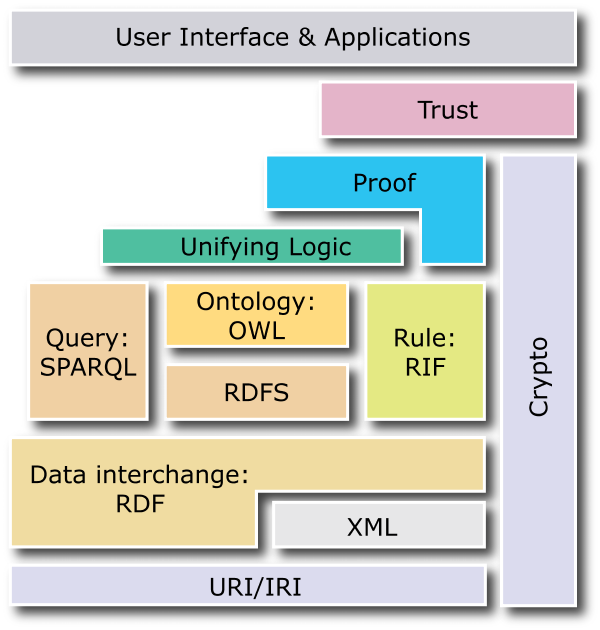
\includegraphics[width=11cm]{figures/SemWebStack}
\caption{Architektura Sémantického webu (navrhl vynálezce WWW Tim Berners-Lee \cite{semWebStack}). (Zdroj \cite{semWeb})}
\label{diagram:SemWebArch}
\end{center}
\end{figure}

\begin{figure}[h]
\begin{center}
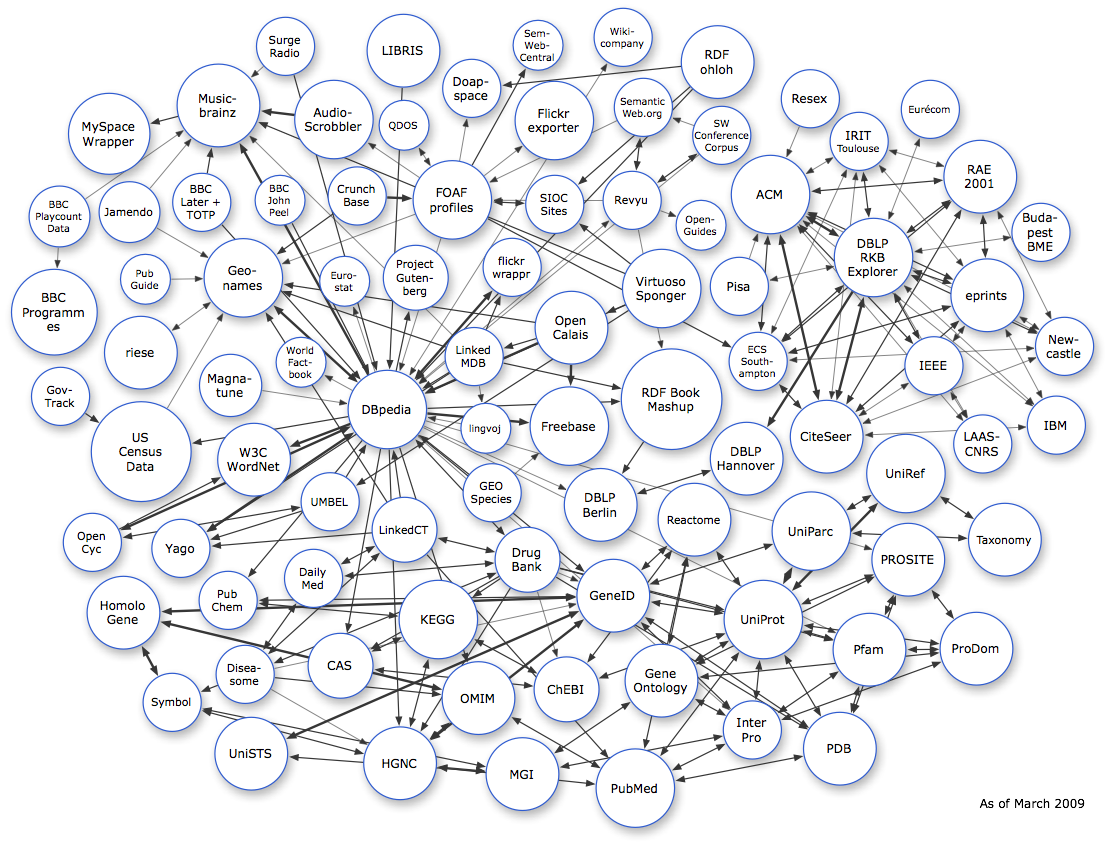
\includegraphics[width=17cm]{figures/linkeddata}
\caption{Graf ontologií (cloud diagram) projektu Linked Data. (Zdroj \cite{linkedData})}
\label{img:linkeddata}
\end{center}
\end{figure}

\begin{figure}[h]
\begin{center}
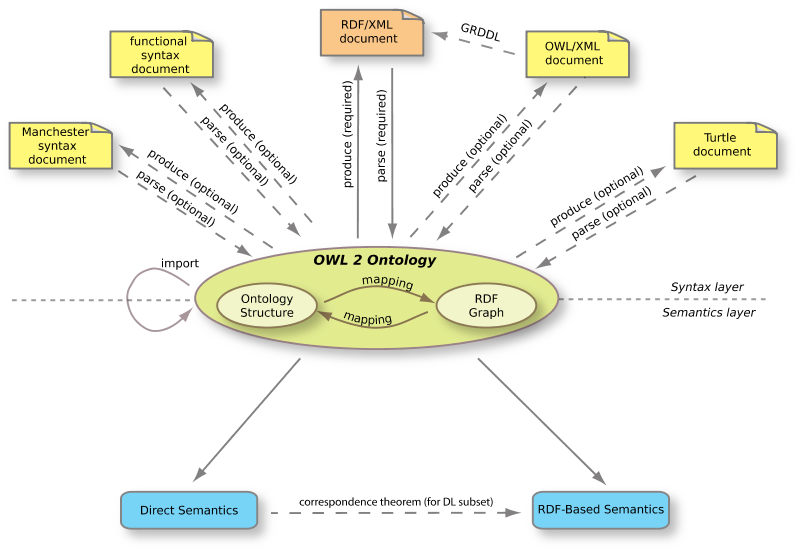
\includegraphics[width=15cm]{figures/OWL2-structure}
\caption{Struktura OWL 2. (Zdroj \cite{owl2})}
\label{img:owl2}
\end{center}
\end{figure}

\begin{figure}[h]
\begin{center}
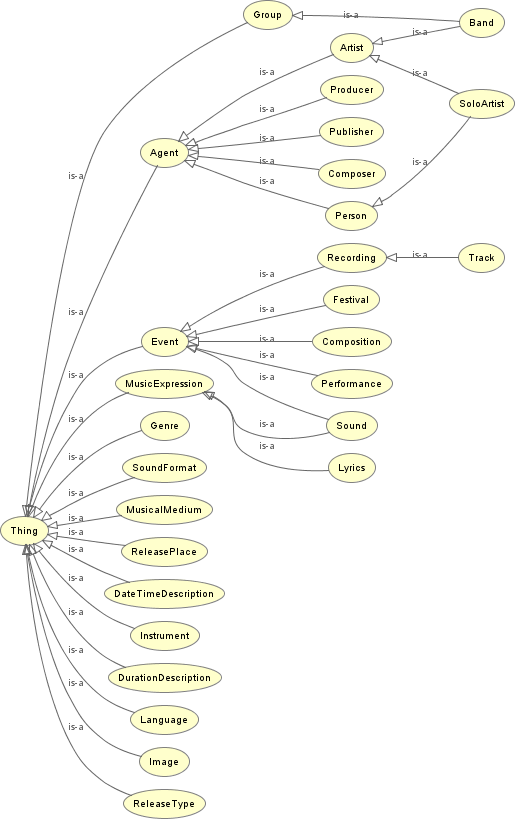
\includegraphics[width=13cm]{figures/mpo_without_genres_instruments}
\caption{Výsledná podoba navržené ontologie (bez hudebních nástrojů a žánrů).}
\label{img:ontoFinal}
\end{center}
\end{figure}

\begin{figure}[h]
\begin{center}
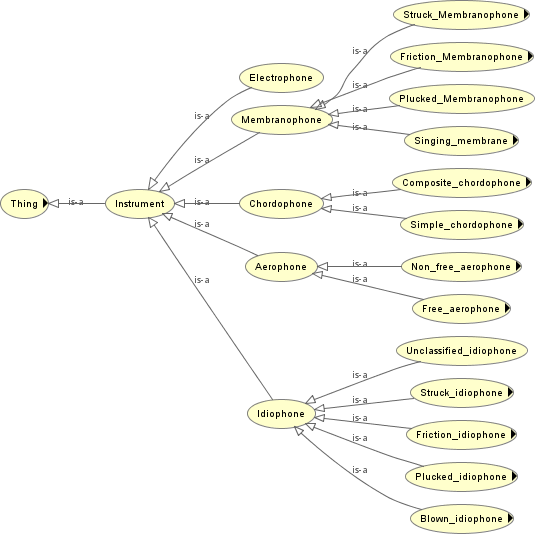
\includegraphics[width=13cm]{figures/mpo_instruments}
\caption{Část struktury tříd hudebních nástrojů podle hudební klasifikace Hornbostel-Sachs.}
\label{img:ontoFinalInstruments}
\end{center}
\end{figure}

\begin{figure}[h]
\begin{center}
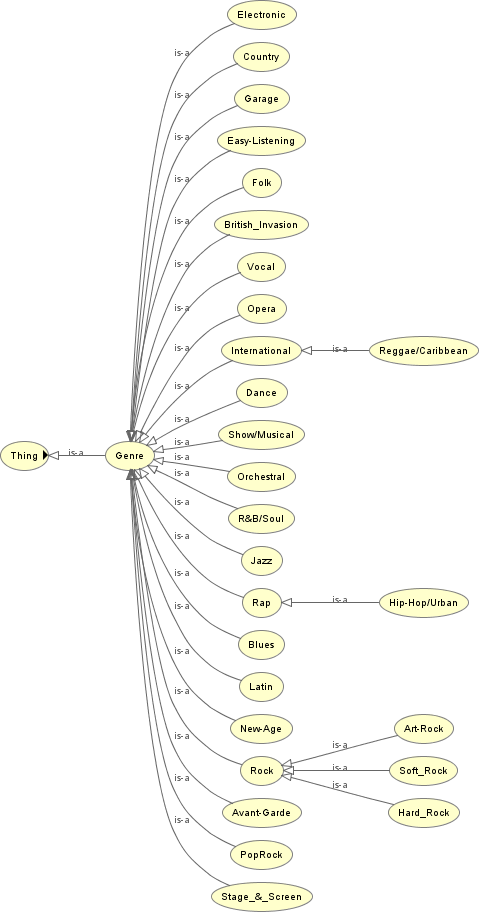
\includegraphics[width=13cm]{figures/mpo_genres}
\caption{Struktura tříd hudebních žánrů.}
\label{img:ontoFinalGenres}
\end{center}
\end{figure}

%*****************************************************************************
\chapter{Instalační příručka}
\textbf{\large Tato příloha velmi žádoucí zejména u softwarových implementačních prací.}


%*****************************************************************************
\chapter{Uživatelská příručka}
\textbf{\large Tato příloha velmi žádoucí zejména u softwarových implementačních prací.}


%*****************************************************************************
\chapter{Obsah přiloženého CD}

Přiložené CD obsahuje veškeré soubory, které jsou součástí tohoto projektu.

\begin{itemize}
\item MusicPlayerOntology/ - kompletní zdrojové kódy webové aplikace včetně ontologie
\item OWLDoc/ - dokumentace ontologie vygenerovaná pluginem OWLDoc
\item text/ - text bakalářské práce + zdrojové soubory pro LaTeX
\end{itemize}

\end{document}
